%%%%%%%%%%%%%%%%%%%%%%%%%%%%%% -*- Mode: Latex -*- %%%%%%%%%%%%%%%%%%%%%%%%%%%%
%% 05-03.tex -- IEEE Software Paper on Software Development Stream.
%% Author          : Hongbing Kou
%% Created On      : Mon Sep 23 11:52:28 2002
%% Last Modified By: Philip M. Johnson
%% Last Modified On: Wed Jul 13 09:59:47 2005
%% RCS: $Id$
%%%%%%%%%%%%%%%%%%%%%%%%%%%%%%%%%%%%%%%%%%%%%%%%%%%%%%%%%%%%%%%%%%%%%%%%%%%%%%%
%%   Copyright (C) 2005 Hongbing Kou
%%%%%%%%%%%%%%%%%%%%%%%%%%%%%%%%%%%%%%%%%%%%%%%%%%%%%%%%%%%%%%%%%%%%%%%%%%%%%%%
%% 

\documentclass[11pt,twocolumn]{article} 
% Psfig/TeX 
\def\PsfigVersion{1.9}
% dvips version
%
% All psfig/tex software, documentation, and related files
% in this distribution of psfig/tex are 
% Copyright 1987, 1988, 1991 Trevor J. Darrell
%
% Permission is granted for use and non-profit distribution of psfig/tex 
% providing that this notice is clearly maintained. The right to
% distribute any portion of psfig/tex for profit or as part of any commercial
% product is specifically reserved for the author(s) of that portion.
%
% *** Feel free to make local modifications of psfig as you wish,
% *** but DO NOT post any changed or modified versions of ``psfig''
% *** directly to the net. Send them to me and I'll try to incorporate
% *** them into future versions. If you want to take the psfig code 
% *** and make a new program (subject to the copyright above), distribute it, 
% *** (and maintain it) that's fine, just don't call it psfig.
%
% Bugs and improvements to trevor@media.mit.edu.
%
% Thanks to Greg Hager (GDH) and Ned Batchelder for their contributions
% to the original version of this project.
%
% Modified by J. Daniel Smith on 9 October 1990 to accept the
% %%BoundingBox: comment with or without a space after the colon.  Stole
% file reading code from Tom Rokicki's EPSF.TEX file (see below).
%
% More modifications by J. Daniel Smith on 29 March 1991 to allow the
% the included PostScript figure to be rotated.  The amount of
% rotation is specified by the "angle=" parameter of the \psfig command.
%
% Modified by Robert Russell on June 25, 1991 to allow users to specify
% .ps filenames which don't yet exist, provided they explicitly provide
% boundingbox information via the \psfig command. Note: This will only work
% if the "file=" parameter follows all four "bb???=" parameters in the
% command. This is due to the order in which psfig interprets these params.
%
%  3 Jul 1991	JDS	check if file already read in once
%  4 Sep 1991	JDS	fixed incorrect computation of rotated
%			bounding box
% 25 Sep 1991	GVR	expanded synopsis of \psfig
% 14 Oct 1991	JDS	\fbox code from LaTeX so \psdraft works with TeX
%			changed \typeout to \ps@typeout
% 17 Oct 1991	JDS	added \psscalefirst and \psrotatefirst
%

% From: gvr@cs.brown.edu (George V. Reilly)
%
% \psdraft	draws an outline box, but doesn't include the figure
%		in the DVI file.  Useful for previewing.
%
% \psfull	includes the figure in the DVI file (default).
%
% \psscalefirst width= or height= specifies the size of the figure
% 		before rotation.
% \psrotatefirst (default) width= or height= specifies the size of the
% 		 figure after rotation.  Asymetric figures will
% 		 appear to shrink.
%
% \psfigurepath#1	sets the path to search for the figure
%
% \psfig
% usage: \psfig{file=, figure=, height=, width=,
%			bbllx=, bblly=, bburx=, bbury=,
%			rheight=, rwidth=, clip=, angle=, silent=}
%
%	"file" is the filename.  If no path name is specified and the
%		file is not found in the current directory,
%		it will be looked for in directory \psfigurepath.
%	"figure" is a synonym for "file".
%	By default, the width and height of the figure are taken from
%		the BoundingBox of the figure.
%	If "width" is specified, the figure is scaled so that it has
%		the specified width.  Its height changes proportionately.
%	If "height" is specified, the figure is scaled so that it has
%		the specified height.  Its width changes proportionately.
%	If both "width" and "height" are specified, the figure is scaled
%		anamorphically.
%	"bbllx", "bblly", "bburx", and "bbury" control the PostScript
%		BoundingBox.  If these four values are specified
%               *before* the "file" option, the PSFIG will not try to
%               open the PostScript file.
%	"rheight" and "rwidth" are the reserved height and width
%		of the figure, i.e., how big TeX actually thinks
%		the figure is.  They default to "width" and "height".
%	The "clip" option ensures that no portion of the figure will
%		appear outside its BoundingBox.  "clip=" is a switch and
%		takes no value, but the `=' must be present.
%	The "angle" option specifies the angle of rotation (degrees, ccw).
%	The "silent" option makes \psfig work silently.
%

% check to see if macros already loaded in (maybe some other file says
% "\input psfig") ...
\ifx\undefined\psfig\else\endinput\fi

%
% from a suggestion by eijkhout@csrd.uiuc.edu to allow
% loading as a style file. Changed to avoid problems
% with amstex per suggestion by jbence@math.ucla.edu

\let\LaTeXAtSign=\@
\let\@=\relax
\edef\psfigRestoreAt{\catcode`\@=\number\catcode`@\relax}
%\edef\psfigRestoreAt{\catcode`@=\number\catcode`@\relax}
\catcode`\@=11\relax
\newwrite\@unused
\def\ps@typeout#1{{\let\protect\string\immediate\write\@unused{#1}}}
\ps@typeout{psfig/tex \PsfigVersion}

%% Here's how you define your figure path.  Should be set up with null
%% default and a user useable definition.

\def\figurepath{./}
\def\psfigurepath#1{\edef\figurepath{#1}}

%
% @psdo control structure -- similar to Latex @for.
% I redefined these with different names so that psfig can
% be used with TeX as well as LaTeX, and so that it will not 
% be vunerable to future changes in LaTeX's internal
% control structure,
%
\def\@nnil{\@nil}
\def\@empty{}
\def\@psdonoop#1\@@#2#3{}
\def\@psdo#1:=#2\do#3{\edef\@psdotmp{#2}\ifx\@psdotmp\@empty \else
    \expandafter\@psdoloop#2,\@nil,\@nil\@@#1{#3}\fi}
\def\@psdoloop#1,#2,#3\@@#4#5{\def#4{#1}\ifx #4\@nnil \else
       #5\def#4{#2}\ifx #4\@nnil \else#5\@ipsdoloop #3\@@#4{#5}\fi\fi}
\def\@ipsdoloop#1,#2\@@#3#4{\def#3{#1}\ifx #3\@nnil 
       \let\@nextwhile=\@psdonoop \else
      #4\relax\let\@nextwhile=\@ipsdoloop\fi\@nextwhile#2\@@#3{#4}}
\def\@tpsdo#1:=#2\do#3{\xdef\@psdotmp{#2}\ifx\@psdotmp\@empty \else
    \@tpsdoloop#2\@nil\@nil\@@#1{#3}\fi}
\def\@tpsdoloop#1#2\@@#3#4{\def#3{#1}\ifx #3\@nnil 
       \let\@nextwhile=\@psdonoop \else
      #4\relax\let\@nextwhile=\@tpsdoloop\fi\@nextwhile#2\@@#3{#4}}
% 
% \fbox is defined in latex.tex; so if \fbox is undefined, assume that
% we are not in LaTeX.
% Perhaps this could be done better???
\ifx\undefined\fbox
% \fbox code from modified slightly from LaTeX
\newdimen\fboxrule
\newdimen\fboxsep
\newdimen\ps@tempdima
\newbox\ps@tempboxa
\fboxsep = 3pt
\fboxrule = .4pt
\long\def\fbox#1{\leavevmode\setbox\ps@tempboxa\hbox{#1}\ps@tempdima\fboxrule
    \advance\ps@tempdima \fboxsep \advance\ps@tempdima \dp\ps@tempboxa
   \hbox{\lower \ps@tempdima\hbox
  {\vbox{\hrule height \fboxrule
          \hbox{\vrule width \fboxrule \hskip\fboxsep
          \vbox{\vskip\fboxsep \box\ps@tempboxa\vskip\fboxsep}\hskip 
                 \fboxsep\vrule width \fboxrule}
                 \hrule height \fboxrule}}}}
\fi
%
%%%%%%%%%%%%%%%%%%%%%%%%%%%%%%%%%%%%%%%%%%%%%%%%%%%%%%%%%%%%%%%%%%%
% file reading stuff from epsf.tex
%   EPSF.TEX macro file:
%   Written by Tomas Rokicki of Radical Eye Software, 29 Mar 1989.
%   Revised by Don Knuth, 3 Jan 1990.
%   Revised by Tomas Rokicki to accept bounding boxes with no
%      space after the colon, 18 Jul 1990.
%   Portions modified/removed for use in PSFIG package by
%      J. Daniel Smith, 9 October 1990.
%
\newread\ps@stream
\newif\ifnot@eof       % continue looking for the bounding box?
\newif\if@noisy        % report what you're making?
\newif\if@atend        % %%BoundingBox: has (at end) specification
\newif\if@psfile       % does this look like a PostScript file?
%
% PostScript files should start with `%!'
%
{\catcode`\%=12\global\gdef\epsf@start{%!}}
\def\epsf@PS{PS}
%
\def\epsf@getbb#1{%
%
%   The first thing we need to do is to open the
%   PostScript file, if possible.
%
\openin\ps@stream=#1
\ifeof\ps@stream\ps@typeout{Error, File #1 not found}\else
%
%   Okay, we got it. Now we'll scan lines until we find one that doesn't
%   start with %. We're looking for the bounding box comment.
%
   {\not@eoftrue \chardef\other=12
    \def\do##1{\catcode`##1=\other}\dospecials \catcode`\ =10
    \loop
       \if@psfile
	  \read\ps@stream to \epsf@fileline
       \else{
	  \obeyspaces
          \read\ps@stream to \epsf@tmp\global\let\epsf@fileline\epsf@tmp}
       \fi
       \ifeof\ps@stream\not@eoffalse\else
%
%   Check the first line for `%!'.  Issue a warning message if its not
%   there, since the file might not be a PostScript file.
%
       \if@psfile\else
       \expandafter\epsf@test\epsf@fileline:. \\%
       \fi
%
%   We check to see if the first character is a % sign;
%   if so, we look further and stop only if the line begins with
%   `%%BoundingBox:' and the `(atend)' specification was not found.
%   That is, the only way to stop is when the end of file is reached,
%   or a `%%BoundingBox: llx lly urx ury' line is found.
%
          \expandafter\epsf@aux\epsf@fileline:. \\%
       \fi
   \ifnot@eof\repeat
   }\closein\ps@stream\fi}%
%
% This tests if the file we are reading looks like a PostScript file.
%
\long\def\epsf@test#1#2#3:#4\\{\def\epsf@testit{#1#2}
			\ifx\epsf@testit\epsf@start\else
\ps@typeout{Warning! File does not start with `\epsf@start'.  It may not be a PostScript file.}
			\fi
			\@psfiletrue} % don't test after 1st line
%
%   We still need to define the tricky \epsf@aux macro. This requires
%   a couple of magic constants for comparison purposes.
%
{\catcode`\%=12\global\let\epsf@percent=%\global\def\epsf@bblit{%BoundingBox}}
%
%
%   So we're ready to check for `%BoundingBox:' and to grab the
%   values if they are found.  We continue searching if `(at end)'
%   was found after the `%BoundingBox:'.
%
\long\def\epsf@aux#1#2:#3\\{\ifx#1\epsf@percent
   \def\epsf@testit{#2}\ifx\epsf@testit\epsf@bblit
	\@atendfalse
        \epsf@atend #3 . \\%
	\if@atend	
	   \if@verbose{
		\ps@typeout{psfig: found `(atend)'; continuing search}
	   }\fi
        \else
        \epsf@grab #3 . . . \\%
        \not@eoffalse
        \global\no@bbfalse
        \fi
   \fi\fi}%
%
%   Here we grab the values and stuff them in the appropriate definitions.
%
\def\epsf@grab #1 #2 #3 #4 #5\\{%
   \global\def\epsf@llx{#1}\ifx\epsf@llx\empty
      \epsf@grab #2 #3 #4 #5 .\\\else
   \global\def\epsf@lly{#2}%
   \global\def\epsf@urx{#3}\global\def\epsf@ury{#4}\fi}%
%
% Determine if the stuff following the %%BoundingBox is `(atend)'
% J. Daniel Smith.  Copied from \epsf@grab above.
%
\def\epsf@atendlit{(atend)} 
\def\epsf@atend #1 #2 #3\\{%
   \def\epsf@tmp{#1}\ifx\epsf@tmp\empty
      \epsf@atend #2 #3 .\\\else
   \ifx\epsf@tmp\epsf@atendlit\@atendtrue\fi\fi}


% End of file reading stuff from epsf.tex
%%%%%%%%%%%%%%%%%%%%%%%%%%%%%%%%%%%%%%%%%%%%%%%%%%%%%%%%%%%%%%%%%%%

%%%%%%%%%%%%%%%%%%%%%%%%%%%%%%%%%%%%%%%%%%%%%%%%%%%%%%%%%%%%%%%%%%%
% trigonometry stuff from "trig.tex"
\chardef\psletter = 11 % won't conflict with \begin{letter} now...
\chardef\other = 12

\newif \ifdebug %%% turn me on to see TeX hard at work ...
\newif\ifc@mpute %%% don't need to compute some values
\c@mputetrue % but assume that we do

\let\then = \relax
\def\r@dian{pt }
\let\r@dians = \r@dian
\let\dimensionless@nit = \r@dian
\let\dimensionless@nits = \dimensionless@nit
\def\internal@nit{sp }
\let\internal@nits = \internal@nit
\newif\ifstillc@nverging
\def \Mess@ge #1{\ifdebug \then \message {#1} \fi}

{ %%% Things that need abnormal catcodes %%%
	\catcode `\@ = \psletter
	\gdef \nodimen {\expandafter \n@dimen \the \dimen}
	\gdef \term #1 #2 #3%
	       {\edef \t@ {\the #1}%%% freeze parameter 1 (count, by value)
		\edef \t@@ {\expandafter \n@dimen \the #2\r@dian}%
				   %%% freeze parameter 2 (dimen, by value)
		\t@rm {\t@} {\t@@} {#3}%
	       }
	\gdef \t@rm #1 #2 #3%
	       {{%
		\count 0 = 0
		\dimen 0 = 1 \dimensionless@nit
		\dimen 2 = #2\relax
		\Mess@ge {Calculating term #1 of \nodimen 2}%
		\loop
		\ifnum	\count 0 < #1
		\then	\advance \count 0 by 1
			\Mess@ge {Iteration \the \count 0 \space}%
			\Multiply \dimen 0 by {\dimen 2}%
			\Mess@ge {After multiplication, term = \nodimen 0}%
			\Divide \dimen 0 by {\count 0}%
			\Mess@ge {After division, term = \nodimen 0}%
		\repeat
		\Mess@ge {Final value for term #1 of 
				\nodimen 2 \space is \nodimen 0}%
		\xdef \Term {#3 = \nodimen 0 \r@dians}%
		\aftergroup \Term
	       }}
	\catcode `\p = \other
	\catcode `\t = \other
	\gdef \n@dimen #1pt{#1} %%% throw away the ``pt''
}

\def \Divide #1by #2{\divide #1 by #2} %%% just a synonym

\def \Multiply #1by #2%%% allows division of a dimen by a dimen
       {{%%% should really freeze parameter 2 (dimen, passed by value)
	\count 0 = #1\relax
	\count 2 = #2\relax
	\count 4 = 65536
	\Mess@ge {Before scaling, count 0 = \the \count 0 \space and
			count 2 = \the \count 2}%
	\ifnum	\count 0 > 32767 %%% do our best to avoid overflow
	\then	\divide \count 0 by 4
		\divide \count 4 by 4
	\else	\ifnum	\count 0 < -32767
		\then	\divide \count 0 by 4
			\divide \count 4 by 4
		\else
		\fi
	\fi
	\ifnum	\count 2 > 32767 %%% while retaining reasonable accuracy
	\then	\divide \count 2 by 4
		\divide \count 4 by 4
	\else	\ifnum	\count 2 < -32767
		\then	\divide \count 2 by 4
			\divide \count 4 by 4
		\else
		\fi
	\fi
	\multiply \count 0 by \count 2
	\divide \count 0 by \count 4
	\xdef \product {#1 = \the \count 0 \internal@nits}%
	\aftergroup \product
       }}

\def\r@duce{\ifdim\dimen0 > 90\r@dian \then   % sin(x+90) = sin(180-x)
		\multiply\dimen0 by -1
		\advance\dimen0 by 180\r@dian
		\r@duce
	    \else \ifdim\dimen0 < -90\r@dian \then  % sin(-x) = sin(360+x)
		\advance\dimen0 by 360\r@dian
		\r@duce
		\fi
	    \fi}

\def\Sine#1%
       {{%
	\dimen 0 = #1 \r@dian
	\r@duce
	\ifdim\dimen0 = -90\r@dian \then
	   \dimen4 = -1\r@dian
	   \c@mputefalse
	\fi
	\ifdim\dimen0 = 90\r@dian \then
	   \dimen4 = 1\r@dian
	   \c@mputefalse
	\fi
	\ifdim\dimen0 = 0\r@dian \then
	   \dimen4 = 0\r@dian
	   \c@mputefalse
	\fi
%
	\ifc@mpute \then
        	% convert degrees to radians
		\divide\dimen0 by 180
		\dimen0=3.141592654\dimen0
%
		\dimen 2 = 3.1415926535897963\r@dian %%% a well-known constant
		\divide\dimen 2 by 2 %%% we only deal with -pi/2 : pi/2
		\Mess@ge {Sin: calculating Sin of \nodimen 0}%
		\count 0 = 1 %%% see power-series expansion for sine
		\dimen 2 = 1 \r@dian %%% ditto
		\dimen 4 = 0 \r@dian %%% ditto
		\loop
			\ifnum	\dimen 2 = 0 %%% then we've done
			\then	\stillc@nvergingfalse 
			\else	\stillc@nvergingtrue
			\fi
			\ifstillc@nverging %%% then calculate next term
			\then	\term {\count 0} {\dimen 0} {\dimen 2}%
				\advance \count 0 by 2
				\count 2 = \count 0
				\divide \count 2 by 2
				\ifodd	\count 2 %%% signs alternate
				\then	\advance \dimen 4 by \dimen 2
				\else	\advance \dimen 4 by -\dimen 2
				\fi
		\repeat
	\fi		
			\xdef \sine {\nodimen 4}%
       }}

% Now the Cosine can be calculated easily by calling \Sine
\def\Cosine#1{\ifx\sine\UnDefined\edef\Savesine{\relax}\else
		             \edef\Savesine{\sine}\fi
	{\dimen0=#1\r@dian\advance\dimen0 by 90\r@dian
	 \Sine{\nodimen 0}
	 \xdef\cosine{\sine}
	 \xdef\sine{\Savesine}}}	      
% end of trig stuff
%%%%%%%%%%%%%%%%%%%%%%%%%%%%%%%%%%%%%%%%%%%%%%%%%%%%%%%%%%%%%%%%%%%%

\def\psdraft{
	\def\@psdraft{0}
	%\ps@typeout{draft level now is \@psdraft \space . }
}
\def\psfull{
	\def\@psdraft{100}
	%\ps@typeout{draft level now is \@psdraft \space . }
}

\psfull

\newif\if@scalefirst
\def\psscalefirst{\@scalefirsttrue}
\def\psrotatefirst{\@scalefirstfalse}
\psrotatefirst

\newif\if@draftbox
\def\psnodraftbox{
	\@draftboxfalse
}
\def\psdraftbox{
	\@draftboxtrue
}
\@draftboxtrue

\newif\if@prologfile
\newif\if@postlogfile
\def\pssilent{
	\@noisyfalse
}
\def\psnoisy{
	\@noisytrue
}
\psnoisy
%%% These are for the option list.
%%% A specification of the form a = b maps to calling \@p@@sa{b}
\newif\if@bbllx
\newif\if@bblly
\newif\if@bburx
\newif\if@bbury
\newif\if@height
\newif\if@width
\newif\if@rheight
\newif\if@rwidth
\newif\if@angle
\newif\if@clip
\newif\if@verbose
\def\@p@@sclip#1{\@cliptrue}


\newif\if@decmpr

%%% GDH 7/26/87 -- changed so that it first looks in the local directory,
%%% then in a specified global directory for the ps file.
%%% RPR 6/25/91 -- changed so that it defaults to user-supplied name if
%%% boundingbox info is specified, assuming graphic will be created by
%%% print time.
%%% TJD 10/19/91 -- added bbfile vs. file distinction, and @decmpr flag

\def\@p@@sfigure#1{\def\@p@sfile{null}\def\@p@sbbfile{null}
	        \openin1=#1.bb
		\ifeof1\closein1
	        	\openin1=\figurepath#1.bb
			\ifeof1\closein1
			        \openin1=#1
				\ifeof1\closein1%
				       \openin1=\figurepath#1
					\ifeof1
					   \ps@typeout{Error, File #1 not found}
						\if@bbllx\if@bblly
				   		\if@bburx\if@bbury
			      				\def\@p@sfile{#1}%
			      				\def\@p@sbbfile{#1}%
							\@decmprfalse
				  	   	\fi\fi\fi\fi
					\else\closein1
				    		\def\@p@sfile{\figurepath#1}%
				    		\def\@p@sbbfile{\figurepath#1}%
						\@decmprfalse
	                       		\fi%
			 	\else\closein1%
					\def\@p@sfile{#1}
					\def\@p@sbbfile{#1}
					\@decmprfalse
			 	\fi
			\else
				\def\@p@sfile{\figurepath#1}
				\def\@p@sbbfile{\figurepath#1.bb}
				\@decmprtrue
			\fi
		\else
			\def\@p@sfile{#1}
			\def\@p@sbbfile{#1.bb}
			\@decmprtrue
		\fi}

\def\@p@@sfile#1{\@p@@sfigure{#1}}

\def\@p@@sbbllx#1{
		%\ps@typeout{bbllx is #1}
		\@bbllxtrue
		\dimen100=#1
		\edef\@p@sbbllx{\number\dimen100}
}
\def\@p@@sbblly#1{
		%\ps@typeout{bblly is #1}
		\@bbllytrue
		\dimen100=#1
		\edef\@p@sbblly{\number\dimen100}
}
\def\@p@@sbburx#1{
		%\ps@typeout{bburx is #1}
		\@bburxtrue
		\dimen100=#1
		\edef\@p@sbburx{\number\dimen100}
}
\def\@p@@sbbury#1{
		%\ps@typeout{bbury is #1}
		\@bburytrue
		\dimen100=#1
		\edef\@p@sbbury{\number\dimen100}
}
\def\@p@@sheight#1{
		\@heighttrue
		\dimen100=#1
   		\edef\@p@sheight{\number\dimen100}
		%\ps@typeout{Height is \@p@sheight}
}
\def\@p@@swidth#1{
		%\ps@typeout{Width is #1}
		\@widthtrue
		\dimen100=#1
		\edef\@p@swidth{\number\dimen100}
}
\def\@p@@srheight#1{
		%\ps@typeout{Reserved height is #1}
		\@rheighttrue
		\dimen100=#1
		\edef\@p@srheight{\number\dimen100}
}
\def\@p@@srwidth#1{
		%\ps@typeout{Reserved width is #1}
		\@rwidthtrue
		\dimen100=#1
		\edef\@p@srwidth{\number\dimen100}
}
\def\@p@@sangle#1{
		%\ps@typeout{Rotation is #1}
		\@angletrue
%		\dimen100=#1
		\edef\@p@sangle{#1} %\number\dimen100}
}
\def\@p@@ssilent#1{ 
		\@verbosefalse
}
\def\@p@@sprolog#1{\@prologfiletrue\def\@prologfileval{#1}}
\def\@p@@spostlog#1{\@postlogfiletrue\def\@postlogfileval{#1}}
\def\@cs@name#1{\csname #1\endcsname}
\def\@setparms#1=#2,{\@cs@name{@p@@s#1}{#2}}
%
% initialize the defaults (size the size of the figure)
%
\def\ps@init@parms{
		\@bbllxfalse \@bbllyfalse
		\@bburxfalse \@bburyfalse
		\@heightfalse \@widthfalse
		\@rheightfalse \@rwidthfalse
		\def\@p@sbbllx{}\def\@p@sbblly{}
		\def\@p@sbburx{}\def\@p@sbbury{}
		\def\@p@sheight{}\def\@p@swidth{}
		\def\@p@srheight{}\def\@p@srwidth{}
		\def\@p@sangle{0}
		\def\@p@sfile{} \def\@p@sbbfile{}
		\def\@p@scost{10}
		\def\@sc{}
		\@prologfilefalse
		\@postlogfilefalse
		\@clipfalse
		\if@noisy
			\@verbosetrue
		\else
			\@verbosefalse
		\fi
}
%
% Go through the options setting things up.
%
\def\parse@ps@parms#1{
	 	\@psdo\@psfiga:=#1\do
		   {\expandafter\@setparms\@psfiga,}}
%
% Compute bb height and width
%
\newif\ifno@bb
\def\bb@missing{
	\if@verbose{
		\ps@typeout{psfig: searching \@p@sbbfile \space  for bounding box}
	}\fi
	\no@bbtrue
	\epsf@getbb{\@p@sbbfile}
        \ifno@bb \else \bb@cull\epsf@llx\epsf@lly\epsf@urx\epsf@ury\fi
}	
\def\bb@cull#1#2#3#4{
	\dimen100=#1 bp\edef\@p@sbbllx{\number\dimen100}
	\dimen100=#2 bp\edef\@p@sbblly{\number\dimen100}
	\dimen100=#3 bp\edef\@p@sbburx{\number\dimen100}
	\dimen100=#4 bp\edef\@p@sbbury{\number\dimen100}
	\no@bbfalse
}
% rotate point (#1,#2) about (0,0).
% The sine and cosine of the angle are already stored in \sine and
% \cosine.  The result is placed in (\p@intvaluex, \p@intvaluey).
\newdimen\p@intvaluex
\newdimen\p@intvaluey
\def\rotate@#1#2{{\dimen0=#1 sp\dimen1=#2 sp
%            	calculate x' = x \cos\theta - y \sin\theta
		  \global\p@intvaluex=\cosine\dimen0
		  \dimen3=\sine\dimen1
		  \global\advance\p@intvaluex by -\dimen3
% 		calculate y' = x \sin\theta + y \cos\theta
		  \global\p@intvaluey=\sine\dimen0
		  \dimen3=\cosine\dimen1
		  \global\advance\p@intvaluey by \dimen3
		  }}
\def\compute@bb{
		\no@bbfalse
		\if@bbllx \else \no@bbtrue \fi
		\if@bblly \else \no@bbtrue \fi
		\if@bburx \else \no@bbtrue \fi
		\if@bbury \else \no@bbtrue \fi
		\ifno@bb \bb@missing \fi
		\ifno@bb \ps@typeout{FATAL ERROR: no bb supplied or found}
			\no-bb-error
		\fi
		%
%\ps@typeout{BB: \@p@sbbllx, \@p@sbblly, \@p@sbburx, \@p@sbbury} 
%
% store height/width of original (unrotated) bounding box
		\count203=\@p@sbburx
		\count204=\@p@sbbury
		\advance\count203 by -\@p@sbbllx
		\advance\count204 by -\@p@sbblly
		\edef\ps@bbw{\number\count203}
		\edef\ps@bbh{\number\count204}
		%\ps@typeout{ psbbh = \ps@bbh, psbbw = \ps@bbw }
		\if@angle 
			\Sine{\@p@sangle}\Cosine{\@p@sangle}
	        	{\dimen100=\maxdimen\xdef\r@p@sbbllx{\number\dimen100}
					    \xdef\r@p@sbblly{\number\dimen100}
			                    \xdef\r@p@sbburx{-\number\dimen100}
					    \xdef\r@p@sbbury{-\number\dimen100}}
%
% Need to rotate all four points and take the X-Y extremes of the new
% points as the new bounding box.
                        \def\minmaxtest{
			   \ifnum\number\p@intvaluex<\r@p@sbbllx
			      \xdef\r@p@sbbllx{\number\p@intvaluex}\fi
			   \ifnum\number\p@intvaluex>\r@p@sbburx
			      \xdef\r@p@sbburx{\number\p@intvaluex}\fi
			   \ifnum\number\p@intvaluey<\r@p@sbblly
			      \xdef\r@p@sbblly{\number\p@intvaluey}\fi
			   \ifnum\number\p@intvaluey>\r@p@sbbury
			      \xdef\r@p@sbbury{\number\p@intvaluey}\fi
			   }
%			lower left
			\rotate@{\@p@sbbllx}{\@p@sbblly}
			\minmaxtest
%			upper left
			\rotate@{\@p@sbbllx}{\@p@sbbury}
			\minmaxtest
%			lower right
			\rotate@{\@p@sbburx}{\@p@sbblly}
			\minmaxtest
%			upper right
			\rotate@{\@p@sbburx}{\@p@sbbury}
			\minmaxtest
			\edef\@p@sbbllx{\r@p@sbbllx}\edef\@p@sbblly{\r@p@sbblly}
			\edef\@p@sbburx{\r@p@sbburx}\edef\@p@sbbury{\r@p@sbbury}
%\ps@typeout{rotated BB: \r@p@sbbllx, \r@p@sbblly, \r@p@sbburx, \r@p@sbbury}
		\fi
		\count203=\@p@sbburx
		\count204=\@p@sbbury
		\advance\count203 by -\@p@sbbllx
		\advance\count204 by -\@p@sbblly
		\edef\@bbw{\number\count203}
		\edef\@bbh{\number\count204}
		%\ps@typeout{ bbh = \@bbh, bbw = \@bbw }
}
%
% \in@hundreds performs #1 * (#2 / #3) correct to the hundreds,
%	then leaves the result in @result
%
\def\in@hundreds#1#2#3{\count240=#2 \count241=#3
		     \count100=\count240	% 100 is first digit #2/#3
		     \divide\count100 by \count241
		     \count101=\count100
		     \multiply\count101 by \count241
		     \advance\count240 by -\count101
		     \multiply\count240 by 10
		     \count101=\count240	%101 is second digit of #2/#3
		     \divide\count101 by \count241
		     \count102=\count101
		     \multiply\count102 by \count241
		     \advance\count240 by -\count102
		     \multiply\count240 by 10
		     \count102=\count240	% 102 is the third digit
		     \divide\count102 by \count241
		     \count200=#1\count205=0
		     \count201=\count200
			\multiply\count201 by \count100
		 	\advance\count205 by \count201
		     \count201=\count200
			\divide\count201 by 10
			\multiply\count201 by \count101
			\advance\count205 by \count201
			%
		     \count201=\count200
			\divide\count201 by 100
			\multiply\count201 by \count102
			\advance\count205 by \count201
			%
		     \edef\@result{\number\count205}
}
\def\compute@wfromh{
		% computing : width = height * (bbw / bbh)
		\in@hundreds{\@p@sheight}{\@bbw}{\@bbh}
		%\ps@typeout{ \@p@sheight * \@bbw / \@bbh, = \@result }
		\edef\@p@swidth{\@result}
		%\ps@typeout{w from h: width is \@p@swidth}
}
\def\compute@hfromw{
		% computing : height = width * (bbh / bbw)
	        \in@hundreds{\@p@swidth}{\@bbh}{\@bbw}
		%\ps@typeout{ \@p@swidth * \@bbh / \@bbw = \@result }
		\edef\@p@sheight{\@result}
		%\ps@typeout{h from w : height is \@p@sheight}
}
\def\compute@handw{
		\if@height 
			\if@width
			\else
				\compute@wfromh
			\fi
		\else 
			\if@width
				\compute@hfromw
			\else
				\edef\@p@sheight{\@bbh}
				\edef\@p@swidth{\@bbw}
			\fi
		\fi
}
\def\compute@resv{
		\if@rheight \else \edef\@p@srheight{\@p@sheight} \fi
		\if@rwidth \else \edef\@p@srwidth{\@p@swidth} \fi
		%\ps@typeout{rheight = \@p@srheight, rwidth = \@p@srwidth}
}
%		
% Compute any missing values
\def\compute@sizes{
	\compute@bb
	\if@scalefirst\if@angle
% at this point the bounding box has been adjsuted correctly for
% rotation.  PSFIG does all of its scaling using \@bbh and \@bbw.  If
% a width= or height= was specified along with \psscalefirst, then the
% width=/height= value needs to be adjusted to match the new (rotated)
% bounding box size (specifed in \@bbw and \@bbh).
%    \ps@bbw       width=
%    -------  =  ---------- 
%    \@bbw       new width=
% so `new width=' = (width= * \@bbw) / \ps@bbw; where \ps@bbw is the
% width of the original (unrotated) bounding box.
	\if@width
	   \in@hundreds{\@p@swidth}{\@bbw}{\ps@bbw}
	   \edef\@p@swidth{\@result}
	\fi
	\if@height
	   \in@hundreds{\@p@sheight}{\@bbh}{\ps@bbh}
	   \edef\@p@sheight{\@result}
	\fi
	\fi\fi
	\compute@handw
	\compute@resv}

%
% \psfig
% usage : \psfig{file=, height=, width=, bbllx=, bblly=, bburx=, bbury=,
%			rheight=, rwidth=, clip=}
%
% "clip=" is a switch and takes no value, but the `=' must be present.
\def\psfig#1{\vbox {
	% do a zero width hard space so that a single
	% \psfig in a centering enviornment will behave nicely
	%{\setbox0=\hbox{\ }\ \hskip-\wd0}
	%
	\ps@init@parms
	\parse@ps@parms{#1}
	\compute@sizes
	%
	\ifnum\@p@scost<\@psdraft{
		%
		\special{ps::[begin] 	\@p@swidth \space \@p@sheight \space
				\@p@sbbllx \space \@p@sbblly \space
				\@p@sbburx \space \@p@sbbury \space
				startTexFig \space }
		\if@angle
			\special {ps:: \@p@sangle \space rotate \space} 
		\fi
		\if@clip{
			\if@verbose{
				\ps@typeout{(clip)}
			}\fi
			\special{ps:: doclip \space }
		}\fi
		\if@prologfile
		    \special{ps: plotfile \@prologfileval \space } \fi
		\if@decmpr{
			\if@verbose{
				\ps@typeout{psfig: including \@p@sfile.Z \space }
			}\fi
			\special{ps: plotfile "`zcat \@p@sfile.Z" \space }
		}\else{
			\if@verbose{
				\ps@typeout{psfig: including \@p@sfile \space }
			}\fi
			\special{ps: plotfile \@p@sfile \space }
		}\fi
		\if@postlogfile
		    \special{ps: plotfile \@postlogfileval \space } \fi
		\special{ps::[end] endTexFig \space }
		% Create the vbox to reserve the space for the figure.
		\vbox to \@p@srheight sp{
		% 1/92 TJD Changed from "true sp" to "sp" for magnification.
			\hbox to \@p@srwidth sp{
				\hss
			}
		\vss
		}
	}\else{
		% draft figure, just reserve the space and print the
		% path name.
		\if@draftbox{		
			% Verbose draft: print file name in box
			\hbox{\frame{\vbox to \@p@srheight sp{
			\vss
			\hbox to \@p@srwidth sp{ \hss \@p@sfile \hss }
			\vss
			}}}
		}\else{
			% Non-verbose draft
			\vbox to \@p@srheight sp{
			\vss
			\hbox to \@p@srwidth sp{\hss}
			\vss
			}
		}\fi	



	}\fi
}}
\psfigRestoreAt
\let\@=\LaTeXAtSign




\usepackage{/export/home/csdl/tex/icse2003/latex8}
\usepackage{times}
\usepackage{url}
%% A verbatim-like environment which allows font changes
%%\usepackage{alltt}
%% New LaTeX2e graphics support
\usepackage[final]{graphicx}
% uncomment the % away on next line to produce the final camera-ready version
% and uncomment the \thispagestyle{empty} following \maketitle
%\pagestyle{empty}
\begin{document}

\title{Studying Micro-Processes in Software Development Stream}
\author{\protect\begin{tabular}{ccc}
Hongbing Kou \\
\end{tabular}\\
\em  Collaborative Software Development Laboratory \\
\em  Department of Information and Computer Sciences \\
\em  University of Hawai'i \\
\em  Honolulu, HI 96822 \\
\em  hongbing@hawaii.edu}
\maketitle
\thispagestyle{empty}

\begin{abstract}  % 200 words
  In this paper we propose a new streaming technique to study software
  development. As we observed software development consists of a series of
  activities such as edit, compilation, testing, debug and deployment etc.
  All these activities contribute to development stream, which is a
  collection of software development activities in time order. Development
  stream can help us replay and reveal software development process at a
  later time without too much hassle. We developed a system called Zorro to
  generate and analyze development stream at Collaborative Software
  Development Laboratory in University of Hawaii. It is built on the top of
  Hackystat\cite{csdl2-02-07}, an in-process automatic metric collection
  system developed in the CSDL.  Hackystat sensors continuously collect
  development activities and send them to a centralized data store for
  processing. Zorro reads in all data of a project and constructs stream
  from them. Tokenizers are chained together to divide development stream
  into episodes (micro iteration) for classification with rule engine. In
  this paper we demonstrate the analysis on Test-Driven Development (TDD)
  with this framework.
\end{abstract}

\Section{Introduction}
\label{sec:intro}
Software development is a very complex process from requirement analysis to
project deployment. It requires developers understand domain knowledge well
and have enough skills to produce high-quality code following a certain
process. Traditionally this process is heavy and evaluated by standards
such as ISO9001 or Capability Maturity Model (CMM). The recent trend in
software process is agile process, which advocates light incremental
iterative development with rapid feedback. Extreme programming
\cite{Beck:00} is one kind of agile process. Unlike plan-driven processes
such as Rational Unified Process(RUP), Team Software Process (TSP), extreme
programming depends on developers' self-control and internal discipline for
process compliance.  In eXtreme Programming (XP) pair-programming provides
support for process compliance because of pair-pressure and pair-learning
\cite{Williams:00}.  It will entirely depend on individual developer's self
control and discipline while pair-programming is not applied. Personal
Software Process (PSP), the foundation of Team Software Process(TSP)
\cite{Humphrey:99} suffers the same problem as extreme programming because
developers have to stop on-hand work frequently to record process data
manually or semi-automatically, which lowers data quality as Disney and
Johnson discovered \cite{csdl-98-04}.

There are many case studies on Test-Driven Development, one of the core
component of extreme programming. George et al \cite{George:04} and
M\"uller \cite{Muller:02} et al did researches on Test-Driven Development
(TDD) \cite{Beck:03}, one of the central practices of extreme programming.
George et al found that TDD developers produced higher quality code
\cite{George:04} while M\"uller et al concluded TDD does not accelerate the
implementation and improve the product quality \cite{Muller:02}. There are
other studies drew either positive \cite{Olan:03,Edwards:04}, neutral
\cite{Geras:04} or negative \cite{Matjaz:03} conclusion on quality and
productivity. In these experiments, researches conducted the studies based
on their understandings of TDD and test subjects were told to do
Test-Driven Development. Final projects were submitted for comparison study
with projects developed by controlled group.  George et al pointed out that
test subjects had limited training on TDD and pair-programming in their
study \cite{George:04}. Test-Driven Development is very disciplined and
writing test first is not always an easy task even with the help of xUnit
\cite{Beck:03} framework. Discipline of TDD was often ignored in the
experiments, which may deteriorate the conclusions.

Hackystat\cite{csdl2-01-13}, an automatic in-process unobtrusive metric
collection system, was designed and developed to collect development
process data as well as on-going metrics of the artifact being worked on
to lower process data collection overhead. Hackystat sensors
\cite{HackystatSensor} are installed in Integrated Development
Environment(IDE) such as JBuilder, Eclipse and Emacs, and also build
utilities such as ANT, Unix Shell, Version Control System (VCS) and issue
tracking system to collect development process data automatically.  IDE
activities such as file edit, refactoring, unit test execution, debug and
build data etc are all interested data to Hackystat sensors. These data are
sent to the centralized Hackystat server for analyses such as in-time
development management support software telemetry \cite{csdl2-04-11} and
continuous Goal-Question-Metric (cGQM).

We developed a system called Zorro on top of Hackystat to drill down into
fine-grained process data to study micro-process of software development.
In Zorro we generate development stream out of sensor data. The stream is
tokenized and classified for process compliance study.

\section{Related Work}
\label{sec:rel}

\section{System Infrastructure}
\label{sec:sys}
Zorro is built on top of Hackystat platform. Development activity data is
grouped together for development streaming, stream tokenization and episode
classification. Development stream is divided into small episodes with the
help of tokenizer. Each episode is a series of continuous activities that
are isolated by token activities. For instance, test-pass episodes are
created when there is a successful unit test invocation. All development
activities happened between two continuous successful test invocations
belong to this test-pass episode. We evaluate episode with pre-defined
rules using JESS \cite{Friedman-Hill:03} rule engine system.

\subsection{Development Stream}
Hackystat sensors collect both process of software development and state
data of projects. To eclipse IDE sensor collects most development
activities such as new project, open project, new file, file open, file
close, file edit, refactoring, unit test etc. Same kind of activities
are grouped together to make sub development streams. They merge together to
make development stream as shown in figure \ref{fig:Streaming}. Activities
irrelevant to the project are filtered out in merging process.

\begin{figure}[ht] 
  \centering
  \includegraphics[width=0.5\textwidth]{picture/Streaming.eps}
  \caption{Hackystat Sensor Data Streaming}\label{fig:Streaming}
\end{figure} 

Development stream is the collection of all development activities occurred
in chronological order. It is similar to time-series data and real-time
stream because they all consist of a series of data in time order.
Development stream is also different from time-series data because it
consists of heterogeneous activity, different from real-time steam because
each activity has well-defined descriptive data structure. These
differences make classical time-series and stream analysis methods hard to
be applied on development stream. In our work we developed a tokenization
mechanism to divide development stream into micro-processes to simplify
analysis.

\subsection{Stream Tokenization}
Activities in development stream are heterogeneous and each of them can
last from milliseconds to hours. The interval between two consecutive
activities also varies from milliseconds to hours. They make development
stream very irregular and stochastic. Since developers follow different
processes development streams vary from developer to developer. To find
patterns in programming we implemented tokenization system to divide
development stream into micro-processes, which are small programming units.
There are four tokenizers in Zorro.
\begin{itemize}
\item \textit{Commit tokenizer} ends an episode when it encounters a bunch
  of file commit activities. It can be used to inspect what developers do
  before integration.
\item \textit{Command tokenizer} ends an episode when there are some
  consecutive command build activities to deploy system in local
  environment.
\item \textit{Test Pass tokenizer} ends an episode when there are
  successful unit test invocations. We implemented it to find the iterations
  in Test-Driven Development.
\item \textit{Buffer transition tokenizer} starts an episode when it
  encounters consecutive buffer transition activities. It sums what
  developers did to the working buffer.
\end{itemize}

Basically tokenizers abstract development stream for better understanding
of the development process. We applied them on development stream and found
that the iterations are either too big such as commit episode, or too
detailed such as buffer transition episode. In the mean time an iteration
may contain too many kinds of activities to be analyzed. These motivated us
to develop tokenizer chain algorithm to iteratively apply tokenizers on the
development stream. Figure \ref{fig:TokenizerChain} is the tokenization
system data flow. Tokenizer 1 applies on development stream to generate
type 1 episodes. They are passed down to be processed by tokenizer 2 when
there are more activities except for token activities.

\begin{figure}[ht] 
  \centering
  \includegraphics[width=0.5\textwidth]{picture/Tokenization.eps}
  \caption{Development Stream Tokenizer Chain}\label{fig:TokenizerChain}
\end{figure} 

To study Test-Driven Development we put commit, command, test pass and
buffer transition tokenizers in a row to work on development stream
iteratively. At the end the long development stream will be tokenized into
many small episodes that can be classified easily as in figure
\ref{fig:Classification}.

\subsection{Classification of Episode}
Episode includes activities to accomplish a certain task. It defines
iteration in software development such that this approach fits to most
modern software development processes because all of them are iterative. In
Test-Driven Development each iteration is either a new test case
implementation or refactoring if developer follows TDD rational strictly.
Because the assumption may not hold we implemented the tokenizer chain to
make our solution be general enough to most development streams. If the
development stream is not Test-Driven Development we will end up with a
bunch of buffer transition episodes.

Test-Driven Development iteration can be elaborated as following\cite{Beck:03}:
\begin{enumerate}
\item Write the test
\item Write the code
\item Run the automated test
\item Refactor
\item Repeat
\end{enumerate}

Clearly an TDD iteration (cycle) contains one or more test pass iterations
which are either Test-Driven or refactor. In order to fine-tune progress of
work we enhanced Hackystat Eclipse sensor to report not only edit work but
also the on-going metrics changes such as number of methods, number of
statements as well as number of test cases and number of assertion
statement to test class. These fine-grained data make it possible to find
incremental small changes on programs to deduce micro-process iterations
accurately.

Finiate State Machine (FSM) is widely used to study sequential data such as
process execution \cite{Cook:95} or language. It has the advantage to find
the hidden patterns in complicated process. Cook discovered ISPW 6/7
process with RNet, KTAIL, and Markov Method \cite{Cook:95} but it ends with
a complicated process diagram that needs process expert's knowledge to
interpret it. We chose rule-based system over FSM in our study of
Test-Driven Development because TDD emphasizes on small and simple
iteration instead of complex process and our interest is on process
compliance not process discovery.  Rule-based system is also stable in the
existence of noise.

Figure \ref{fig:Classification} is the episode tokenization and
classification algorithm of TDD analysis. 
\begin{figure}[ht] 
  \centering
  \includegraphics[width=0.5\textwidth]{picture/Classification.eps}
  \caption{Episode Classification}\label{fig:Classification}
\end{figure} 

The tokenizer chain on the left has commit, command, test-pass and buffer
transition tokenizers. Commit tokenizer is applied on development stream to
make commit episodes. Each commit episode represents one system integration
after a new feature is added or a bug is fixed. Commit activities in the
episode are stripped off before episode activities are passed to command
tokenizer. Test-pass tokenizer will be applied on command episode to
generate test-pass episodes. We assert activities of test-pass episode into
rule engine to do classification. In figure \ref{fig:Classification} the
left-most command episode contains two sub episodes, TDD and refactor.
Buffer transition tokenizer will be applied on non-classifiable test-pass
episode. In the end we get episode tree out of development stream with this
algorithm.

Developers only make small change to let test pass in TDD. We define rules
to check work both on test code and production code to inspect TDD process.
Figure \ref{fig:Query} is the interaction between Zorro and JESS rule
engine system for episode classification with pre-loaded rules. We assert
development activities in time order into JESS working memory as facts and
run JESS engine to fire up rules. 

\begin{figure}[ht] 
  \centering
  \includegraphics[width=0.5\textwidth]{picture/Query.eps}
  \caption{Classification Query}\label{fig:Query}
\end{figure} 

In Zorro we use term ``action'' to represent development activity, which is
the meta operation in development. Here is the action template definition
in CLIP language for JESS.
\begin{verbatim}
;; Action template.
(deftemplate Action
  "Common parts of all actions"
  (slot index) ;Order in episode
  (slot file)  ;Active file
)
\end{verbatim}

Index is the order of the action in the episode. All actions inherit this
template. We have following actions in Zorro:
\begin{itemize}
\item \textit{Documentation Edit} is the edit action on documentation. It
  has duration inherited from abstract \textit{Edit Action}.
\item \textit{Production Edit Action} is the edit action on production
  code which is java program at present. It defines attributes
  \textit{method change} and \textit{statement change} from the
  incremental work.
\item \textit{Unit Test Edit Action} is the edit action on unit test. It is
  similar to \textit{Production Edit Action} but the work is on unit test
  code. In addition to number of method change and number of statement
  change it includes number of test methods change and number of test
  assertion change too.
\item \textit{Compilation Action} is not compilation invocation but a
  compilation error on the active file..
\item \textit{Unit Test Action} represents an unit test invocation which
  either succeeded or failed. Error message will be attached if it fails.
\item \textit{Buffer Transition Action} is the active buffer's change
  during development.
\item \textit{Unary and Binary Refactor} are two types of refactor
  operators. \textit{Add} and \textit{Delete} are unary while
  \textit{Rename} and \textit{Move} are binary. In addition, refactor
  operation can be on class, import, field or method.
\item \textit{Debug Action} is any debug activity include break pointer
  set/unset, step into, step over etc.
\end{itemize}

\subsection{Test-Driven Development Episode Classification}
Test-Driven Development (TDD) is the way on how to program. Developers
write failed test first before production code. Implementation is driven by
test code and the progress is incremental \cite{Beck:03}.
\begin{quote}
  Red/Green/Refactor is the mantra of Test-Driven Development. It
  implicates the order of programming. 
  \begin{enumerate}
    \item \textit{Red} -- Write a little test that doesn't work, and perhaps
      doesn't even compile at first.
    \item \textit{Green} -- Make the test work quickly, committing whatever
       sins necessary in the process.
    \item \textit{Refactor} -- Eliminate all the duplication created in merely
       getting the test to work.
\end{enumerate}
\end{quote}

Iterations of Test-Driven Development are usually less than ten minutes.
There is no big progress in each iteration except for making test pass.
This iteration can be casted into one to many test-pass episodes. Each
episode will be either a complete TDD iteration or a portion of it.
Episodes of TDD can be either Test-Driven or refactor depends on test
progress.

\subsubsection{Test-Driven Episode}
In a test-driven episode developer writes a test based on requirement
analysis. The test may not even compile at first because the test target
does not exist yet. There should have compilation failure if developer
compiles it or project was configured to be compiled automatically.
Production code is created to get rid of compilation error.  Execution of
this test will probably fail when developer invokes it, which is the red
bar pattern. The rest work of this episode is to have just enough code to
make test pass. This is the scenario of a typical test-driven episode. Even
though developers can be required to follow typical test-driven strictly it
is lame to have this discipline requirement. In some cases there is no
point to let developer do it rigiously.
\begin{itemize}
\item Test code compilation will definitely fail because it tests
  non-existed object or method.
\item The production code to make test pass is trivial. Generating a fake
  implementation to make test fail will be just a waste.
\end{itemize}

The key to TDD is the test case creation and the substantial work to make
test pass. They are the skeleton of a test-driven episode. Depending on the
existence of compilation error and test failure, a test-driven episode can
be one of them in figure \ref{fig:TDD}.

\begin{figure}[ht] 
  \centering
  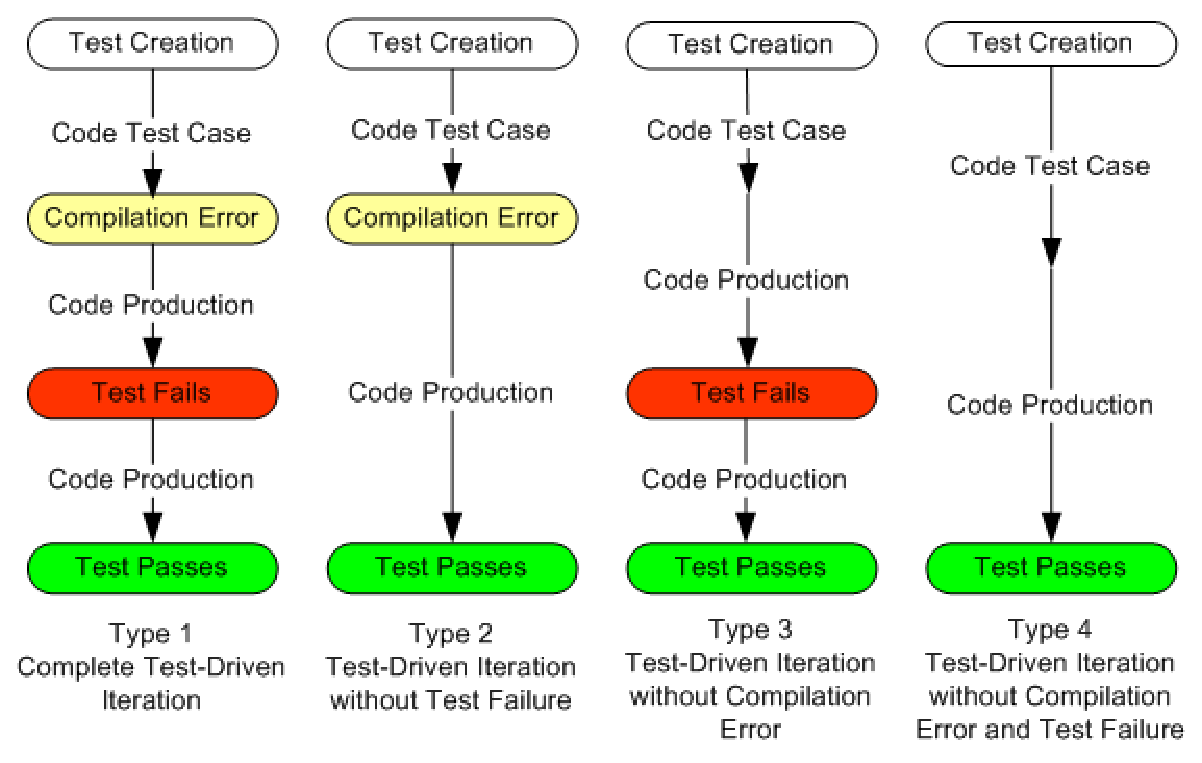
\includegraphics[width=0.5\textwidth]{picture/TDD.eps}
  \caption{Test-Driven Episode Classification}\label{fig:TDD}
\end{figure} 

\subsubsection{Refactor Episode}
Refactoring is the term describes operation to alter a program's internal
structure without changing its external behaviors in software development
\cite{Refactoring}. New feature is introduced by new test cases in TDD such
that an test-pass episode is refactoring as long there is no new test.
Refactoring episode also has four types. In one side refactor can happen
either to test code or production. On another side refactoring operation
may or may not fail the existed tests. Figure \ref{fig:Refactor} depicts
the algorithm of this categorization. In types 3 and 4 there may have some
work on test code without new test created.

\begin{figure}[ht] 
  \centering
  \includegraphics[width=0.5\textwidth]{picture/Refactoring.eps}
  \caption{Test-Driven Refactor Classification}\label{fig:Refactor}
\end{figure} 

\subsubsection{Test-Last Episode and Validation Episode}
Ideally all test-pass episodes are either test-driven or refactor in
Test-Driven Development. The allowance is that developer may create
multiple test cases for the production code to test various inputs. We call
this Test-Last Development contrary to Test-Driven Development in that test
code is created after production code. It is also the canonical programming
habit of most non-TDD developers. Regression or validation is to run the
existed tests to make sure system work well, which happens very often in
software development especially in TDD since test cases from TDD serve as
regression test suite as well. A test episode is validation as long as
there is no substantial edit work on both production and test code.

\subsubsection{Complicated Test-Pass Episode}
TDD advocates developers write a simple test only each time and write
enough code to make failed test pass without committing big bulk of code at
once. This is the discipline required by TDD. It's also called Test-First
Design because test cases define the interaction of the system with
external code delegated by test code in development. In actual project
development developers may breach this discipline because it is tedious to
run unit tests in every small step. Our survey indicates that developers
tend to run tests when they worry that system might break because of the
new code. Although it is not welcomed by TDD we can not stop developers
making big progress. In our study we claim a test-pass episode not
classifiable and complexity high if there are more than two different
production files. This kind of complicated test-pass episode is flagged and
passed down to buffer transition tokenizer for further investigation.

\subsubsection{Classification of Buffer Transition Episode}
Buffer transition episode includes developer's activities on the working
buffer. When a test-pass episode is complicated we apply buffer transition
tokenizer on it to deduce developer's work.
\begin{itemize}
\item \textit{Read} -- There are only buffer transition activities in the
  episode.
\item \textit{New} -- There are new class, methods or fields created.
\item \textit{Delete} -- There are only buffer transition and delete
  activities on either test code or production code.
\item \textit{Edit} -- Edit work on documentation, production code or test
  code.
\item \textit{Test} -- There is failed test invocation with possible edit
  work on test or production code.
\end{itemize}

\section{Experiment and Evaluation}
\label{sec:exp}

\section{Discussion}
\label{sec:disc}

\bibliographystyle{/export/home/csdl/tex/icse2003/latex8}
\bibliography{/export/home/csdl/bib/zorro,/export/home/csdl/bib/tdd,/export/home/csdl/bib/csdl-trs,/export/home/csdl/bib/hackystat,/export/home/csdl/bib/psp}
\end{document}























